%%
%% This is file `sample-xelatex.tex',
%% generated with the docstrip utility.
%%
%% The original source files were:
%%
%% samples.dtx  (with options: `sigconf')
%% 
%% IMPORTANT NOTICE:
%% 
%% For the copyright see the source file.
%% 
%% Any modified versions of this file must be renamed
%% with new filenames distinct from sample-xelatex.tex.
%% 
%% For distribution of the original source see the terms
%% for copying and modification in the file samples.dtx.
%% 
%% This generated file may be distributed as long as the
%% original source files, as listed above, are part of the
%% same distribution. (The sources need not necessarily be
%% in the same archive or directory.)
%%
%% The first command in your LaTeX source must be the \documentclass command.
\documentclass[sigconf]{acmart}
\usepackage{graphicx, subfig}
\usepackage{subfigure}
\usepackage[colorlinks,linkcolor=red,anchorcolor=blue,citecolor=green]{hyperref}
\usepackage[top=2cm, bottom=2cm, left=2cm, right=2cm]{geometry}

\makeatletter
\newif\if@restonecol  
\makeatother  
\let\algorithm\relax  
\let\endalgorithm\relax  
\usepackage[linesnumbered,ruled,vlined]{algorithm2e}%[ruled,vlined]{  
\usepackage{algpseudocode}  
\usepackage{amsmath}  
\renewcommand{\algorithmicrequire}{\textbf{Input:}}  % Use Input in the format of Algorithm  
\renewcommand{\algorithmicensure}{\textbf{Output:}} % Use Output in the format of Algorithm 
\usepackage{color}
\usepackage{multirow}
\usepackage{array}
%%
%% \BibTeX command to typeset BibTeX logo in the docs
\AtBeginDocument{%
  \providecommand\BibTeX{{%
    \normalfont B\kern-0.5em{\scshape i\kern-0.25em b}\kern-0.8em\TeX}}}

%% Rights management information.  This information is sent to you
%% when you complete the rights form.  These commands have SAMPLE
%% values in them; it is your responsibility as an author to replace
%% the commands and values with those provided to you when you
%% complete the rights form.
\setcopyright{acmcopyright}
\copyrightyear{2018}
\acmYear{2018}
\acmDOI{10.1145/1122445.1122456}

%% These commands are for a PROCEEDINGS abstract or paper.
\acmConference[Woodstock '18]{Woodstock '18: ACM Symposium on Neural
  Gaze Detection}{June 03--05, 2018}{Woodstock, NY}
\acmBooktitle{Woodstock '18: ACM Symposium on Neural Gaze Detection,
  June 03--05, 2018, Woodstock, NY}
\acmPrice{15.00}
\acmISBN{978-1-4503-XXXX-X/18/06}


%%
%% Submission ID.
%% Use this when submitting an article to a sponsored event. You'll
%% receive a unique submission ID from the organizers
%% of the event, and this ID should be used as the parameter to this command.
%%\acmSubmissionID{123-A56-BU3}

%%
%% The majority of ACM publications use numbered citations and
%% references.  The command \citestyle{authoryear} switches to the
%% "author year" style.
%%
%% If you are preparing content for an event
%% sponsored by ACM SIGGRAPH, you must use the "author year" style of
%% citations and references.
%% Uncommenting
%% the next command will enable that style.
%%\citestyle{acmauthoryear}

%%
%% end of the preamble, start of the body of the document source.
\begin{document}

%%
%% The "title" command has an optional parameter,
%% allowing the author to define a "short title" to be used in page headers.
\title{An electrode event-based quantum micro-architecture for a superconducting quantum processor}

%%
%% The "author" command and its associated commands are used to define
%% the authors and their affiliations.
%% Of note is the shared affiliation of the first two authors, and the
%% "authornote" and "authornotemark" commands
%% used to denote shared contribution to the research.

% \author{Qi Zhou, Lei Huang, Guo Ping Guo}
% \email{zq953100,HL@mail.ustc.edu.cn, gpguo@ustc.edu.cn}
% \affiliation{%
%   \institution{Unitvercity of science and technology of China}
%   \streetaddress{Jin Zhai Road 96}
%   \city{HeFei}
%   \state{China}
% }


% %%
% %% By default, the full list of authors will be used in the page
% %% headers. Often, this list is too long, and will overlap
% %% other information printed in the page headers. This command allows
% %% the author to define a more concise list
% %% of authors' names for this purpose.
% \renewcommand{\shortauthors}{Zhou, et al.}

%%
%% The abstract is a short summary of the work to be presented in the
%% article.

\maketitle

\begin{abstract}
    The control microarchitecture based on the gate model has been proposed in 
    recent research, bridging the gaps between low-level quantum hardware and 
    quantum algorithms. However, In addition to execute quantum application 
    with high issue rate, the implementation of waveform compensation and 
    waveform calibration of quantum gates are also important for a full stack 
    superconducting quantum processor. To this end, we propose and build a 
    prototype of electrode event-based control microarchitecture for superconducting 
    quantum processor. Two core elements of micro-architecture are : 
    i) electrode event based quantum operation unit, 
    ii) hybrid quantum circuit description scheme with local and global events. 
    The micro-architecture is implemented with Field Programmable Gate Array. 
    We propose a multi-level compilation scheme to generate microarchitecture 
    executable program.
  
  \end{abstract}
  
%%
%% The code below is generated by the tool at http://dl.acm.org/ccs.cfm.
%% Please copy and paste the code instead of the example below.
%%
\begin{CCSXML}
    <ccs2012>
     <concept>
      <concept_id>10010520.10010553.10010562</concept_id>
      <concept_desc>Computer systems organization~Embedded systems</concept_desc>
      <concept_significance>500</concept_significance>
     </concept>
     <concept>
      <concept_id>10010520.10010575.10010755</concept_id>
      <concept_desc>Computer systems organization~Redundancy</concept_desc>
      <concept_significance>300</concept_significance>
     </concept>
     <concept>
      <concept_id>10010520.10010553.10010554</concept_id>
      <concept_desc>Computer systems organization~Robotics</concept_desc>
      <concept_significance>100</concept_significance>
     </concept>
     <concept>
      <concept_id>10003033.10003083.10003095</concept_id>
      <concept_desc>Networks~Network reliability</concept_desc>
      <concept_significance>100</concept_significance>
     </concept>
    </ccs2012>
 \end{CCSXML}
    
\ccsdesc[500]{Computer systems organization~Embedded systems}
\ccsdesc[300]{Computer systems organization~Redundancy}
\ccsdesc{Computer systems organization~Robotics}
\ccsdesc[100]{Networks~Network reliability}

%%
%% Keywords. The author(s) should pick words that accurately describe
%% the work being presented. Separate the keywords with commas.
\keywords{Quantum (micro-) architecture, quantum instruction set architecture, 
superconducting quantum processor}

%% A "teaser" image appears between the author and affiliation
%% information and the body of the document, and typically spans the
%% page.


%%
%% This command processes the author and affiliation and title
%% information and builds the first part of the formatted document.
\section{Introduction}
Quantum computation, a paradigm of computing that is completely different from 
classical methods, shows potential to solving classically intractable computational 
problems in areas such as quantum chemistry, cryptography, machine learning, 
and others. The ideal quantum computer should be composed of a top-down system stack, 
which is roughly divided into the top layer of quantum language and algorithm, 
the middle layer of control hardware and bottom layer of quantum processor. 
Recently, google used a programmable superconducting processor to solve a 
specific computational task, which can be regarded as an experimental 
realization of quantum supremacy. With the rapid progress of quantum processor, 
finding out a general architectural solution of control hardware for bridging 
the gap between quantum language and quantum processor is becoming increasingly urgent.

Since dedicated electronic devices which are used to apply well-defined electrical signals 
on quantum processor introduce high resource consumption, long configuration times, 
and control complexity, which seriously limited the scalability, Fu. etc propose a prototype of 
control microarchitecture (QuMA V2) based on circuit model that translates a set of instructions into the 
interface required by a quantum processor. QuMA V2 can relize quantum circuit with little memory overhead, 
as well as support feedback control, which is important for some quantum algorithms,such as ....(其他组的工作)

However, the hardware constraints of quantum processors pose new challenges to the design of 
quantum computing architecture. On the one hand, the waveform parameters of quantum gates fluctuates due to the 
influence of environmental noise, therefore, supporting waveform calibration is necessary for the full stack 
quantum computing architecture to improve the accuracy of the results of quantum circuit. The execution of quantum 
application should include two steps:  waveform calibration and quantum circuit execution. 
In particular, for some quantum applications that need to determine the rotation angle of quantum gates 
used in the next iterative circuit based on the measurement results, such as QAOA, the quantum computing 
architecture also needs to support new waveform generation. For it is impossible to pre-calibrate and store 
all possible waveforms into the waveform library since the rotation angle is continuous and unpredictable 
for each iteration. Figure~\ref{img} shows the quantum program execution flow. On the other hand, waveform compensation 
method is used to reduce the negative effects of crosstalk of DC pulses, reducing the fidelity of quantum gates. 
Using compensating method means that pulses on qubit become contextual --- dependent on what is being played 
simultaneously on other qubits. 

\begin{figure}[ht]
  \centering
  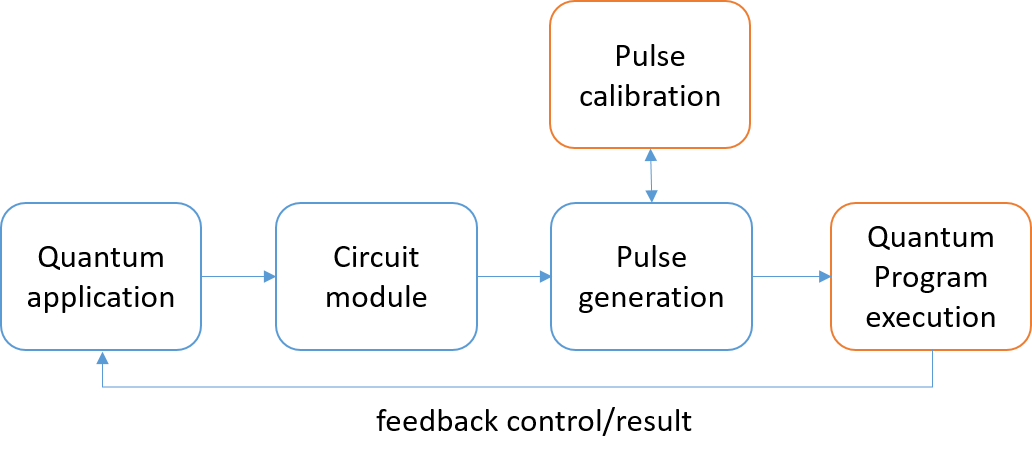
\includegraphics[width=\linewidth]{figure/1}
  \caption{The execution flow of quantum application}
  \label{img}
\end{figure}

The control microarchitecture based on the gate model, that at each timestamp only one pulse for corresponding 
quantum gate act only on the target qubit, is hard to support above two situation. To this end, we propose a quantum control 
micro-architecture based on electrode event, namely ebQuMA. There are three core concepts:
\begin{itemize}
  \item Electrode event based quantum operation unit: The basic unit of quantum operation is the electrode event, which is an abstraction of the waveform applied on one electrode, 
  including waveforms of one quantum gate or a combination of quantum gates over a period of time, 
  calibration experiment and optimized waveform for partial quantum circuit. 
  Each qubit requires multiple types of electrode events that can be applied on the qubit simultaneously, depend on the control architecture of the quantum processor. 
  This solution allows the microarchitecture to control the quantum processor at the electrode level, providing the foundation for supporting calibration experiments and waveform compensation. 
  \item Hybrid event description scheme: Quantum operation instructions are divided into global event 
  operations and local event operations. Local event operations need to specify qubits that execute the event, while global 
  event operations execute the event on all qubits. It provides a simpler description scheme for quantum operations that 
  require compensation, compared with specifying different events for each qubit in turn. In addition, this scheme can 
  also greatly reduce the instruction overhead for the descriptions of the quantum circuit with high gate diversity.
  \item Multi-level compilation scheme: The compilation of quantum application is divided into three steps: compiling 
  the quantum program into a quantum assembly program based on electrode events, generating waveform files for each event, 
  and mapping encoding of each event and the storage address of corresponding waveform. It reduces the task of the 
  microarchitecture at runtime by implementing waveform compensation and waveform generation of high gate diversity 
  circuits at compiling time, thereby improving the issue rate problem.
\end{itemize}

The paper is structured as follows. Section 2 briefly introduces the basics of the control method of superconducting qubits. 
Section 3 presents related previous work. We state the challenges of microarchitecture design 
and our solution with three proposed schemes, respectively in Sections 4 and 5. 
Section 6 discusses the implementation of ebQASM. 
The advantages and resource costs are evaluated in Section 7. 
Section 8 concludes.
\section{Background}
Superconducting quantum computation with the advantage of sufficiently high controllability and low noise is a leading approach in the quantum computing competition.
Many groups including IBM,Google,and Riggetti choose it as a candidate for implementing medium and large-scale quantum computation.
In the paper, our architecture is designed for controlling superconducting quantum chip.
\subsection{control}

\begin{figure}[ht]
  \centering
  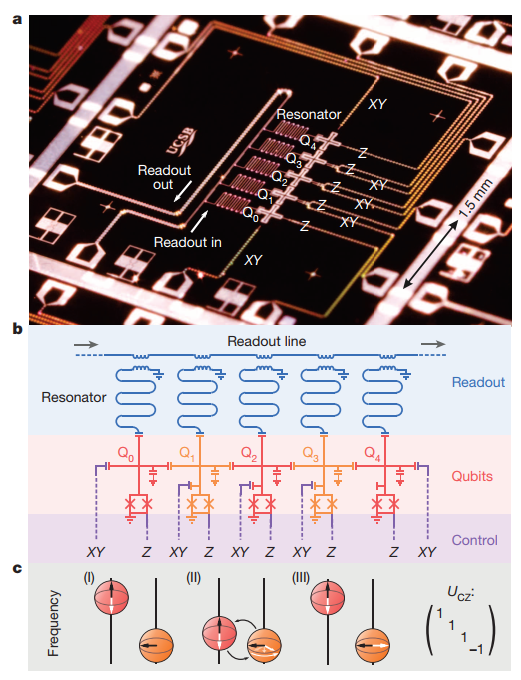
\includegraphics[width=\linewidth]{figure/background}
  \caption{ The quantum circuit based on the gate model and physical implementation}
  \label{imgb}
\end{figure}

Because we focus on how to control quantum chip, not the complex physical processes, 
we abstract quantum chip to an analog circuit and simplify the control problem to a simple process that apply a specific waveform to a specific control line at a specific time.



\ref{imgb} shows the connectivity of qubits and control lines. 
XY lines transfer pulsed microwaves produced by mixing two DAC outputs with a programmable local oscillator. When on resonance with the qubit, XY pulses 
will drive rabi oscillations which can be used to do single qubit gates. 
Z lines transfer static or dynamic voltages which can be used to tune the frequency of qubit and implement two qubit gates by flux biasing the SQUID. 
Readout line transfer pulsed microwaves which are similar to XY lines, but it has two ports that one for waveform input and one for waveform readout. 
When Readout-in waveform is on resonance with resonator, Readout-out waveform will contain status information of qubit.
In this structure, applying a single-qubit operation(like X,Y,H) on qubit is equivalent to apply a set pulsed microwaves on corresponding XY line. 
And similarly, applying a two-qubit operation(like Control-Z) on qubit is to apply a square wave on corresponding Z line.

\subsection{crosstalk}
Because of mutual and self-induction between Z lines, there is crosstalk in the flux biases of two qubits, where flux bias applied to one 
qubit can unintentionally induce flux in other qubits. 
Crosstalk can be regarded as leakage of the control signal and will corrupt the quantum state and lead to incorrect program execution.

For two qubits, crosstalk is expressed in terms of a 2x2 matrix M below.
\[ \begin{bmatrix} Z^r_1 \\ Z^r_2\end{bmatrix}=
\begin{bmatrix} M_1 & m_{12} \\ m_{21}  & M_2 \end{bmatrix} 
\begin{bmatrix} Z_1 \\ Z_2 \end{bmatrix}\]

Where $Z^r_1  $($Z^r_2 $) is the real flux biases of qubit1(qubit2), $Z_1  $($Z_2 $) is the intended flux biases we apply on qubits.In crosstalk matrix, $M_1=M_2=1 $, 
and $m_{12} $ and $m_{21} $ are the crosstalk terms, which are generally not equal to each other.by measuring the frequency change of qubit1(qubit2) with the variation 
of qubit1 Z-pulse and qubit2-Z pluse, We can get the crosstalk matrix.

And then, we can use the crosstalk matrix to make compensation of Z-pulses for reducing the effect of crosstalk.
According to the formula below, $Z_1  $($Z_2 $), the real flux biases needed to apply on Z line, will be inferred from the ideal flux biases $Z_1^{ideal}  $($Z_2^{ideal}  $).
\[\begin{bmatrix} Z_1 \\ Z_2\end{bmatrix}=
{\begin{bmatrix} M_1 & m_{12} \\ m_{21}  & M_2 \end{bmatrix}}^{-1}
\begin{bmatrix} Z_1^{ideal} \\ Z_2^{ideal} \end{bmatrix}\]

It means that the compensation Z-pulses for orthonormalize the control should be applied to all qubits even though we 
only do Z-control on one qubit if consider the effect of crosstalk.
\section{Related works}
So far, there are mainly two quantum processor control architectures: distributed and centralized which adopt different kinds of quantum assembly languages.
A quantum application programmed by quantum high-level language is firstly compiled into quantum assembly language (QASM)-based instructions. 
In addition to converting the quantum application into a circuit model, the compiler also optimizes the types and combinations of quantum gates according to the underlying constraints of the quantum equipment. 
According to the executable degree of quantum assembly language, it is mainly divided into two categories. 

For non-executable QASM, which are mainly intermediate representations of quantum circuit without considering the low-level constraints to interface with the quantum processor, such as QPOL, Quil, and openQASM, 
a distributed architecture is generally used for the control of quantum processor,such as Raytheon BBN APS2 system and the control system of Sycamore, the latest quantum processor of Google. The underlying compiler generates quantum gates sequence of each qubit according to the quantum intermediate representation, 
and converts it into a low-level instructions that can be directly executed by the waveform generation module, such as jump table or waveform address. When the quantum application is executed, 
the central control module triggers each waveform generation module synchronously, which executes low-level instructions and applies the corresponding waveform to each qubit. 
In a word, the central control module is only responsible for scheduling, and waveform splicing and applying are implemented in each waveform generation in the unit of qubit.

Fu. proposed an executable quantum assembly language, which can be directly executed by the centralized control architecture (QuMA\_V2), 
and generating precise control waveform sequences in runtime by instruction execution. 
In the non-deterministic timing domain, the central control module executes instructions based on eQASM and buffers events of quantum gates for each qubit in event queues in the order of execution time points. 
Since the program flow and data transmission can be controlled more flexibly through instructions, this scheme is more suitable for feedback control based on measurement results. On the other hand, 
the deterministic timing domain is controlled by the Timing Controller to trigger buffered events of each qubit when the time point arrived, and the waveform generation module executes events to apply corresponding waveforms. 
In addition to the flexibility, by decoupling the timing of executing instructions and performing output, 
it can maintain fully deterministic timing of the output and maximally process instructions during waiting, providing possibilities for hybrid quantum computing.
\section{microarchitectural challenges}

% \begin{figure*}
%   \begin{minipage}[t]{0.5\textwidth}
%   \centering
%   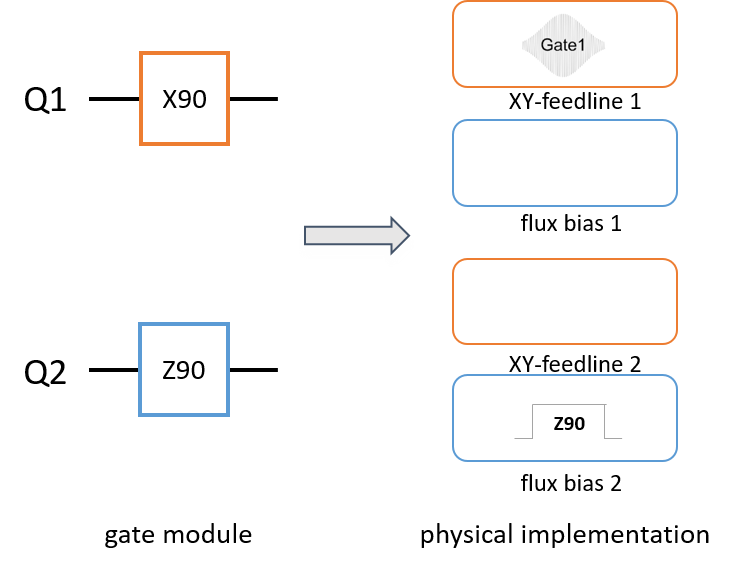
\includegraphics[width=2.2in]{3_1}
%   \caption{fig1}
%   \label{fig:side:a}
%   \end{minipage}%
%   \begin{minipage}[t]{0.5\textwidth}
%   \centering
%   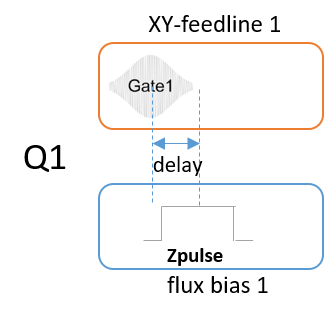
\includegraphics[width=2.2in]{3_4}
%   \caption{fig2}
%   \label{fig:side:b}
%   \end{minipage}
%   \end{figure*}
%   \begin{figure*}
%     \centering
%     \subfigure[Small Box with a Long Caption]{
%       \label{fig:subfig:a} %% label for first subfigure
%       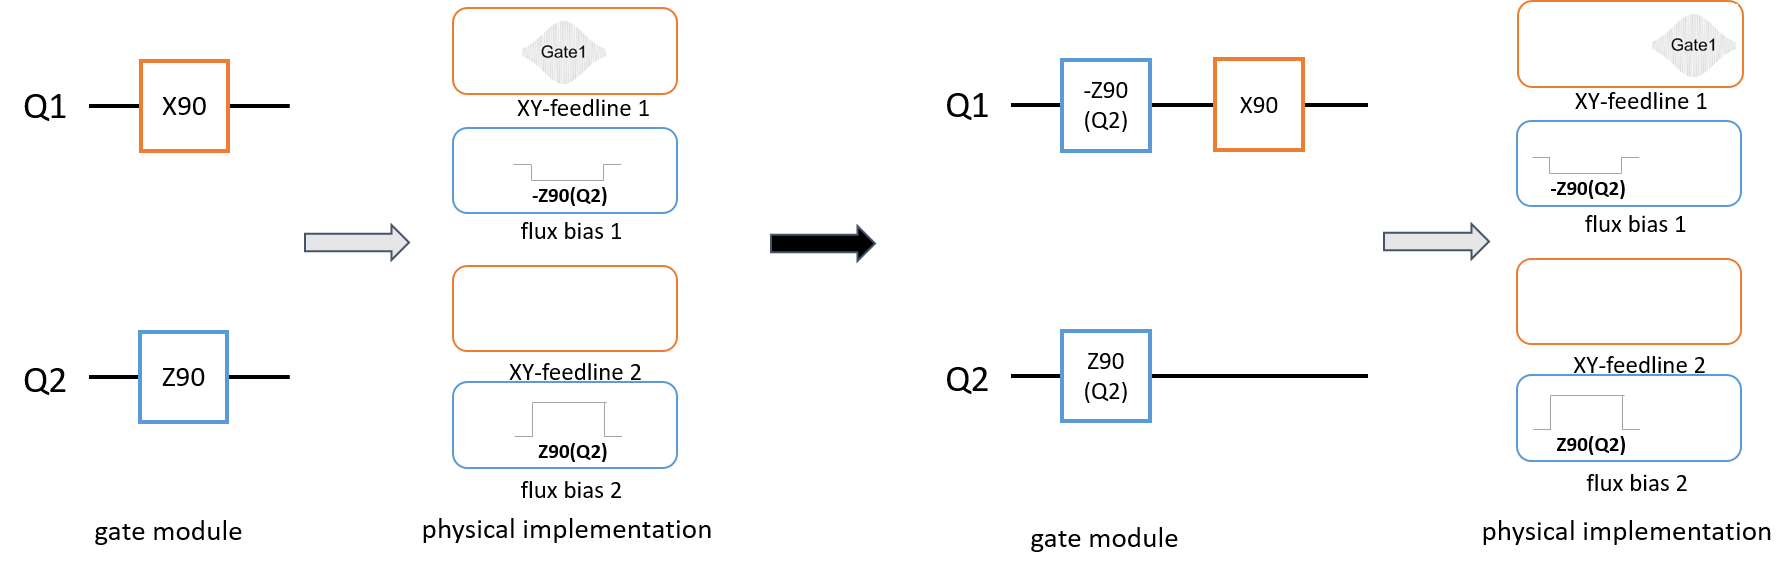
\includegraphics[width=\linewidth]{3_2}}
%     \subfigure[Big Box]{
%       \label{fig:subfig:b} %% label for second subfigure
%       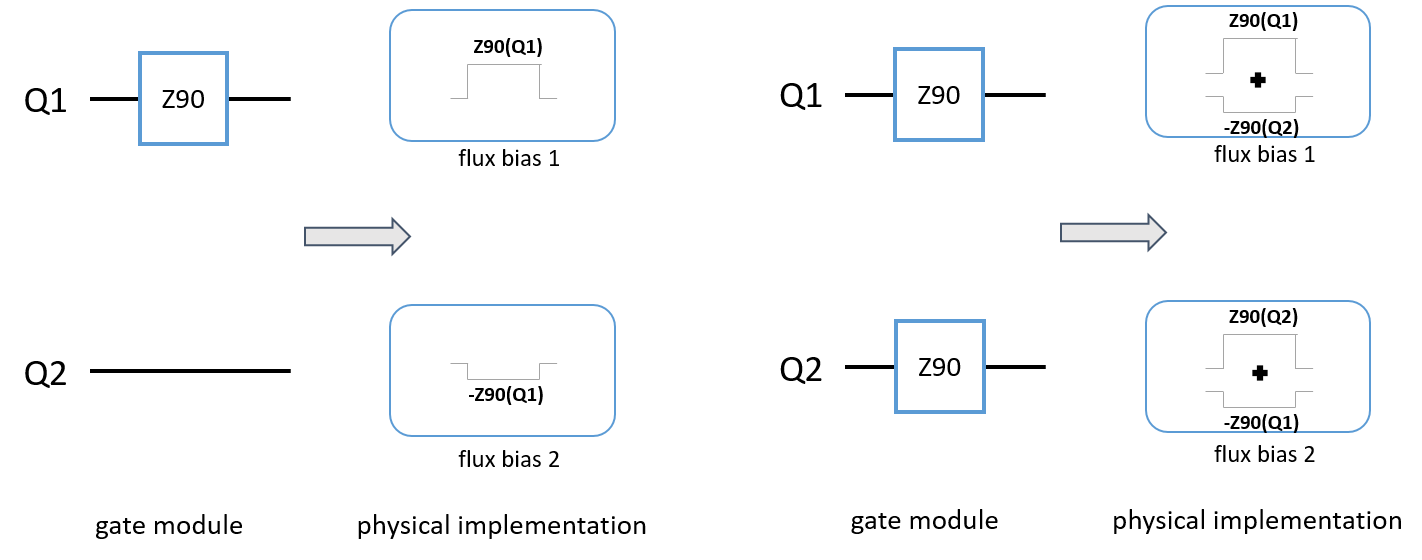
\includegraphics[width=\linewidth]{3_3}}
%     \caption{Two Subfigures}
%     \label{fig:subfig} %% label for entire figure
%   \end{figure*}



\subsection{Limitations Of The Gate Model}
\begin{figure}[ht]
  \centering
  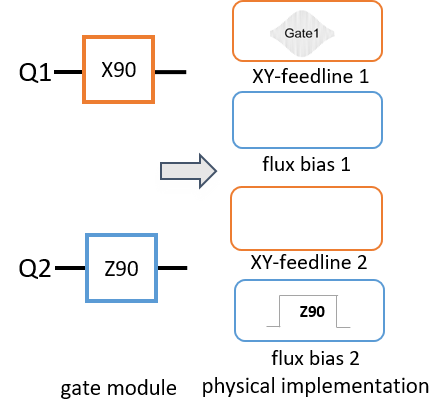
\includegraphics[width=\linewidth]{figure/2_1}
  \caption{The quantum circuit based on the gate model and physical implementation}
  \label{img2_1}
\end{figure}
At present, quantum programs are mainly divided into quantum algorithms and quantum experiments 
(such as RB, allXY), the basic unit of which are quantum gates. In the gate model of quantum computing, 
a program is typically decomposed into a sequence of 1and 2-qubit gates that are realized as control 
pulses acting on corresponding electrode, as shown in Figure~\ref{}. The left side of the figure is a gate model
description of a simple quantum circuit, and the right side is the control practical waveform applied by each 
electrode corresponding to the circuit.

Generally, the controller used to execute quantum programs adopts the gate model to describe 
the quantum program, which greatly reduces the memory consumption and uploading latency of waveform files, 
by combining quantum circuit with basic quantum gates at runtime.However, considering the physical limitations of quantum processors, 
as mentioned in Section 2, the quantum computing architecture requires to support waveform compensation and waveform paramater calibration, 
which is hard to be achieved by the gate model, poseing a challenge for quantum architecture design.

\begin{figure*}[ht]
  \centering
  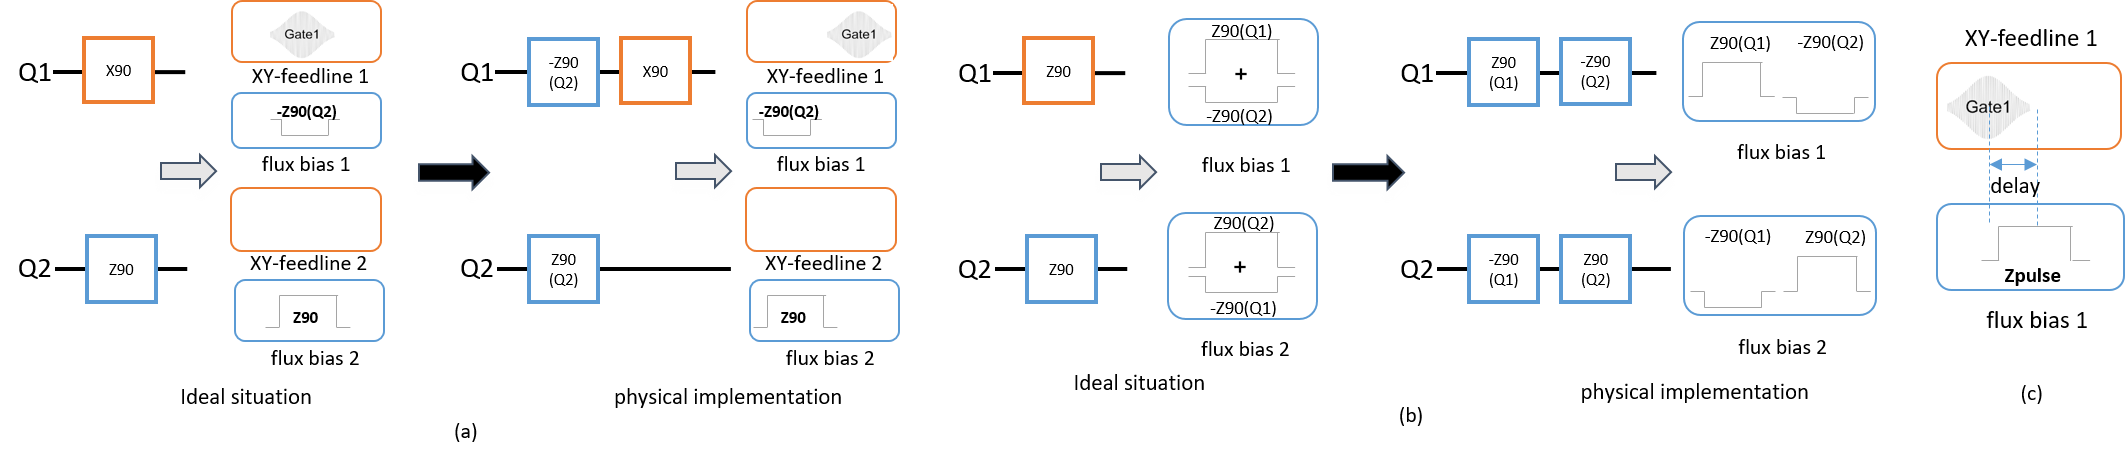
\includegraphics[width=\linewidth]{figure/2_2}
  \caption{Challenges of the gate model}
  \label{img2_2}
\end{figure*}


\subsubsection{Waveform compensation}
Using the gate model to implement waveform compensation increases instruction overhead and reduces the parallelism
of quantum circuits, which limit the scalability of the quantum architecture.

We first consider the case where there is only one compensation gate at one timestamp, 
as shown in Figure 3 (b). At this timestamp, X180 and Z180 are applied to Q1 and Q2, 
respectively. As the two electrodes of Q1 need to apply waveforms at the same time, 
it cannot be described by the gate model. One solution is to execute Z90 Q2 and X180 Q1 in sequence. 
However, it converts efficient parallel circuit into serial one, increasing the depth of circuit. 
On the other hand, when describing the Z180 Q2 in gate model, 
since the rest of qubits require to apply compensation waveforms simultaneously, 
the n-qubit quantum processor needs a total of n operation instructions to implement one compensation gate, 
which greatly increases the complexity of the circuit description and the number of basic logic gates.

For the case where multiple compensation gates are executed at one timestamp, 
as shown in Figure 3 (c), Q1 and Q2 applies Z180 simultaneously, 
since the waveform applied on Q1 is the superposition of the waveforms of Z180 Q1 and the compensation waveform of the Z180 Q2, 
it requires to two different quantum operations to encode Z180 Q1 gate. 
For n-qubit quantum processor, considering all combinations of m types of compensation gates performed at one timestamp, 
each qubit needs to store A waveforms of control operations and B of compensation operations. 
Obviously such a huge number of basic quantum gates are not scalable. 
Although the number of basic gates can be reduced at the cost of the depth of circuit, 
the n compensation gates that are executed simultaneously need to be transformed into n depth circuit, still unacceptable.

\subsubsection{Calibration experiment}
The gate model is not suitable for the description of certain calibration experiments, 
such as the delay calibration experiments between XY pulse and Z pulse. 
Since the latency between the transmission lines of qubits, fluctuating irregularly result from environment noise, 
reduces the fidelity of quantum gates, it is necessary to periodically calibrate the latency and modify the control waveform. 
The experimental waveform is shown in the figure 3 (d). 
The specific experimental scheme can refer to []. 
This experiment requires applying Z pulse and XY pulse to one qubit simultaneously and measuring the final state, contrary to the gate model. 
Therefore, a new circuit description scheme needs to be adopted at the microarchitecture level to support the quantum program execution flow as mentioned in Section1, 
which constitutes a challenge in the design of the quantum architecture.


\subsection{Description Of High Gate Diversity Circuit}
The current quantum programs can mainly divide into two categories: 
the first one is represented by RB algorithm, 
which is characterized by huge circuit depth but small gate density. 
Since the RB algorithm consists of a large number of subroutines, 
the depth of which can be as high as 2000, 
pre-storing all control waveforms will cause large memory overhead and transmission delay. 
Considering each RB program only performs quantum gates on 1-2 qubits, 
it is very suitable to use the gate model description, 
and play the pre-stored waveform of basic quantum gates according to the instructions in runtime.

The second type is used to solve practical problems which requires high-fidelity quantum gates, 
so the depth of circuit is relatively low, 
but the gate density and diversity depend on the specific algorithm.
When the gate diversity is high, it is inefficient to use the gate model. 
Specifically, it can cause serious timing problems when the time overhead of executing quantum 
operation instructions in microarchitecture is greater than the length of corresponding waveforms. 
Recent research has proposed double index quantum vector scheme which support SIMD (same gate, multiple qubits) 
and MIMD (multiple gates, multiple qubits) parallelism in a single instruction to increase the information density of quantum 
operation instructions, but introduces substantial complexity and hardware costs.

Therefore, a new circuit description scheme with satisfying performance for both type of circuits is another important challenge.

\begin{figure*}[ht]
  \centering
  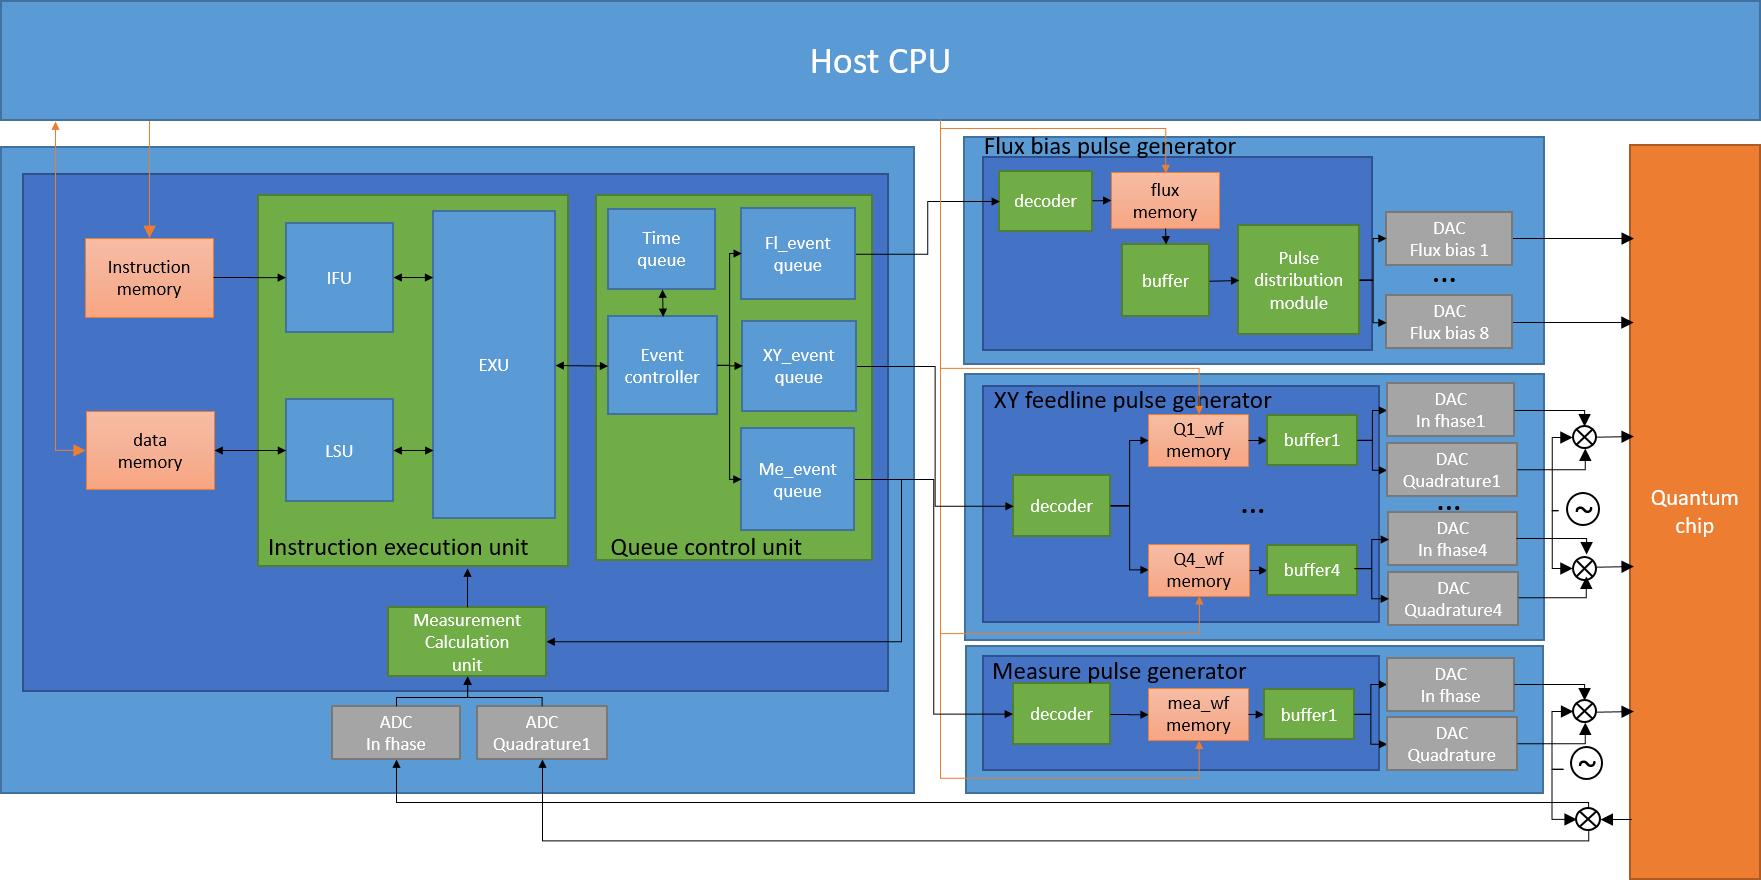
\includegraphics[width=\linewidth]{figure/4_1}
  \caption{overview of electrode event-based microarchitecture}
  \label{img2}
\end{figure*}
\section{quantum microarchitecture}
In this section, we will discuss the electrode event-based quantum microarchitecture as shown in figure~\ref{img2}. 

The input of ebQuMA is generated by the compiler infrastructure, 
which compiles the quantum program 
(including the quantum application described by the gate model and the calibration experiment program) 
into a micro-architecture program coding with ebQIS (electrode event-base Quantum Instruction Set) as shown in table1, 
and generates the waveform file corresponding to each event. 

ebQIS is composed of classic and quantum instructions. 
Classic instructions include arithmetic and logical operations, branch, load and store instructions to support data transferring and program flow control.  
Quantum operation instruction and Qwait are used to describe the electrode events of qubits for each given timestamp, 
and FMR is necessary to obtain the measurement result of qubits. 
In order to increase the information density of the instructions, 
we refer to the VLIW(very long instruction word) and SIMQ(single instruction multiple qubits) schemes proposed by eQASM. 
A quantum operation instruction can contain up to two quantum operations. 

As shown in figure5, the instruction execution unit fetches and executes ebQIS instructions from the instruction memory, performing registers update, program flow control and data communication. 
In particular, quantum operation instructions buffer electrode events with the same timestamp into event registers and send to the queue control unit when a new timestamp arrives. 
The event controller sends the buffered events at the time point specified by the timestamp, to achieve precise time control. 
Pulse generator units obtain the size and address of the waveform according to the encoding of the electrode events, and converts digitally events into corresponding analog pulses by DACs. 
After modulating the output signal of XY feedline and measure pulse generators with radio-frequency carrier waves, 
analog pulses with precise timing can perform quantum operations on qubits. For the measure event, 
in addition to generating measurement waveform, the queue control unit sends the measurement signal to the measurement calculation unit. 
After a fixed delay, the MCU starts to collect the demodulated measurement analog signal, 
obtain the measurement result and send to the instruction execution unit.

We introduce three schemes in ebQuMA to address the challenges described in Section 4.
(i)In ebQIS, The quantum circuit is describing with electrode event based quantum operation. 
By allocating multiple electrode event registers for each qubit, ebQASM supports to apply multiple waveform on different electrode at one timestamp. 
This scheme makes calibration experiments and waveform compensation possible in ebQuMA. 
(ii)electrode events in ebQIS are divided into global and local events, which complement each other. 
The global events can greatly reduce the instruction overhead of circuit description, so as to offset the issue rate problem caused by supporting waveform compensation. 
While local events are used to discribe low gate diversity circuit with high depth to reduce the memory overhead, such as Random Benchmarking.
(iii)In order to support the above two scheme, a multi-level compilation scheme is necessary. The compilation process is divided into three steps. 
Transforming the circuit with gate model into electrode events based description scheme, 
generating waveforms corresponding to each event and micro-architecture program, 
and assigning the coding of each event according to the waveform size and storage address in ebQuMA.

\subsection{Electrode Based Quantum Operation Unit}
First, we propose independent electrode number to characterize the control architecture of different quantum processors. 
The independent electrodes number refers to the category number of independent electrodes required for each qubit to perform all quantum control operations (not including measure operation). 
If one operation requires multiple waveforms superimposed simultaneously, 
since each of them cannot independently implement one operation respectively, 
the number of independent electrodes is still 1(such as XY-rotation operation for superconducting transmon qubit). 
Table 2 shows the independent electrode number of different superconducting quantum processor. 
Although the types and implementation schemes of quantum gates varies, 
In most architecture, two independent electrodes are necessary to implement XY-rotation and Z-rotation \& two-qubit gates, respectively. 
In particular, Google's architecture additionally requires one independent electrode for the coupler.

ebQuMA adopt the electrode event, a abstraction of waveforms on one specific electrode for one qubit, as the basic unit of quantum operation in ebQIS. 
It can be one or combination of multiple quantum gates, or a waveform for calibration experiment and optimized circuit. 
The number of electrode event types depends on the independent electrode number, and distinguished by the encoding of quantum operation. 
Table 3 shows the coding of quantum operation for the quantum processor mentioned in Section 2. 
The quantum circuit in a time period for each qubit is obtained by independent description of different electrode events. 


\begin{algorithm}[ht]
      \caption{caption}
      \begin{ttfamily} 

      \textcolor[RGB]{0,0,205}{ADDI } \quad R1, R0, 40000   \qquad \textcolor[RGB]{169,169,169}{\#cycle number for each measurement}\\
      \textcolor[RGB]{0,0,205}{ADDI } \quad R5, R0, ResultMemAddr\\
      \textcolor[RGB]{0,0,205}{SMIS } \quad S0, 1\\
      \textcolor[RGB]{0,0,205}{ADDI } \quad R2, R0, 0\\
      \textcolor[RGB]{0,0,205}{ADDI } \quad R3, R0, 0\\
      ~\\
      \textcolor[RGB]{34,139,34}{Loop\_1:}\\ 
      \quad 0 , \textcolor[RGB]{139,69,19}{X\_event1} S0 | \textcolor[RGB]{139,69,19}{Z\_event0} S0\\
      \quad 3 , \textcolor[RGB]{139,69,19}{measure} S0\\
      \quad \textcolor[RGB]{0,0,205}{QWAIT} \quad 50\\
      \quad \textcolor[RGB]{0,0,205}{FMR\quad} \quad R4, S0\\
      \quad \textcolor[RGB]{0,0,205}{ADD\quad} \quad R3, R4, R3\\
      \quad \textcolor[RGB]{0,0,205}{ADDI } \quad R2, R2, 1\\
      \quad \textcolor[RGB]{0,0,205}{BNE\quad} \quad R1, R2, \textcolor[RGB]{34,139,34}{Loop\_1}\\
      ~\\
      \textcolor[RGB]{0,0,205}{STORE} \quad R5, R3\\
      \textcolor[RGB]{0,0,205}{ADDI } \quad R3, R0, 0\\
      \textcolor[RGB]{0,0,205}{ADDI } \quad R2, R0, 0\\
      \textcolor[RGB]{0,0,205}{ADDI } \quad R5, R5, 1\\
      ~\\
      \textcolor[RGB]{34,139,34}{Loop\_2:}\\
      \quad 0 , \textcolor[RGB]{139,69,19}{X\_event1} S0 | \textcolor[RGB]{139,69,19}{Z\_event1} S0\\
      \dots

      
      \end{ttfamily} 
\end{algorithm} 

Lower-level control compared with the gate model allows ebQuMA to support calibration experiments.
Figure 5a is a micro-architecture program used to calibrate the timing difference between the microwave drive and flux bias channels based on ebQIS. 
XYevent\_0 corresponds to a $\pi$ pulse and each Zevent corresponds to flattop Z detune shown in figure5b. 
The pulse duration is the same as $\pi$ pulse, while varying the timing between the two. 
The host program can obtain the timing difference from the final state probability of each Zevent and the corresponding delay.

On the other hand, the electrode event can be a waveform of one quantum gate or a combination of quantum gates, which is suitable for the description of quantum circuits with different depth. 
For the quantum circuit shown in Figure 6, we use two different levels abstraction of electrode events to describe. 
One electrode event coding scheme is to encode a combination of all quantum gates of single electrode into one electrode event, and add unitary operation waveforms when no operation applies. 
Correspondingly, the description procedure of this circuit is:\\
\centerline{0,\quad  XYevent\_1 \quad S0 \quad | \quad Zevent\_2 \quad S0;}\\
It only takes one instruction, but require to store the waveform with a total length of 120ns, which includes unitary operation waveforms and repetitive waveforms.

Also, we can take a lower level of abstraction that only encode waveforms of basic quantum gates as electrode events. 
The corresponding procedure is:\\
\centerline{0, \quad XYevent\_2 \quad S0;}\\
\centerline{2, \qquad  Zevent\_3 \quad S0;}\\
\centerline{2, \quad  XYevent\_2 \quad S0;}\\

\begin{figure}[h]
  \centering
  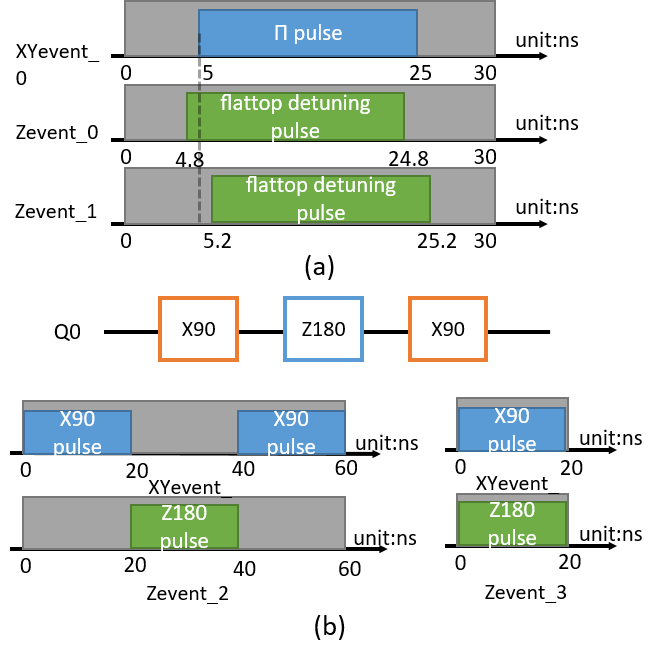
\includegraphics[width=\linewidth]{figure/4_34}
  \caption{overview of electrode event-based microarchitecture}
  \label{img4}
\end{figure}


Although it requires 3 instructions, it only needs to store the waveform of 40ns. 
High level abstraction completes more task of circuit description during the compilation phase instead of runtime, reduces instruction number horizontally
at the cost of memory overhead. The memory resource consumption of this solution will be discussed more in section 8.
In contrast, Lower level abstraction of electrode events greatly reduces memory overhead, which is suitable for the circuit with large depth, such as random benchmarking. 

To support the electrode event-based description scheme, the number of event registers and event queues for each qubit is equivalent to independent electrode number in ebQuMA. 
The instruction execution module buffers quantum operations of different electrodes for each qubit in the corresponding electrode event register when executing the quantum operation instruction, 
and sends the buffered electrode events to the corresponding electrode event queue uniformly when a new timestamp is generated. 
When the queue control unit is triggered and a certain timestamp is reached, 
all electrode events executed at this timestamp are sent to the corresponding waveform generation modules that play the pre-stored waveform synchronously according to the electrode event code.
It is worth noting that since the electrode event is an abstraction of the actual waveform, to adapt different quantum chip architectures, 
the microarchitecture only needs to modify the number of electrode event registers and queues.

\subsection{hybrid Event Description Scheme }
Although the electrode event-based quantum operation unit provides the possibility to implement calibration experiment and waveform compensation, 
it requires to specify the quantum operation applied by each electrode of each qubit for every timestamp. 
Even if we take SOMQ and VLIW schemes, for quantum circuits with large gate diversity, 
such as QV algorithms, and quantum gates required waveform compensation, 
which means every qubit needs to apply a quantum operation (quantum gate waveform or compensation waveform), 
it will still cause serious issue rate problem, especially when qubit number is large. 
To this end, we propose a hybrid event description scheme with local and global events.

The local event requires an operand in mask format to specify the target qubits. Generally, local electrode events are low-level abstractions, 
representation of single quantum gate or calibrated waveform. 
When performing quantum applications, each local event corresponds to one quantum gate, same as the gate model.
By using local event to describe quantum circuit, only basic waveforms need to be stored, but requires more instructions, which is suitable for circuits with lower gate diversity but larger depth. 
For calibration experiments, the local events of each qubit are independent of others, which means they are not valid on every qubit, specified during the compilation phase.

In addition to local events, ebQIS introduces global events, which apply the electrode event on all qubits. 
The types of events are distinguished by the coding of quantum operations, as shown in Table 1. 
Since the global event does not require an operand, the segment corresponding to the operand register is used as an extension segment for the quantum operation encoding, 
providing a larger addressing space for global events.
As all qubits need to perform global events, (no operation qubits play the unitary operation waveform), 
when the gate density is low, more invalid waveform are stored, Resulting in low memory utilization. 
However, for large gate diversity circuit, global events can greatly reduce the number of instructions and avoid issue rate problems. 
In particular, since compensation quantum gates require to apply waveforms on all qubits, they are well-suited for global event coding.

\begin{figure}[h]
  \centering
  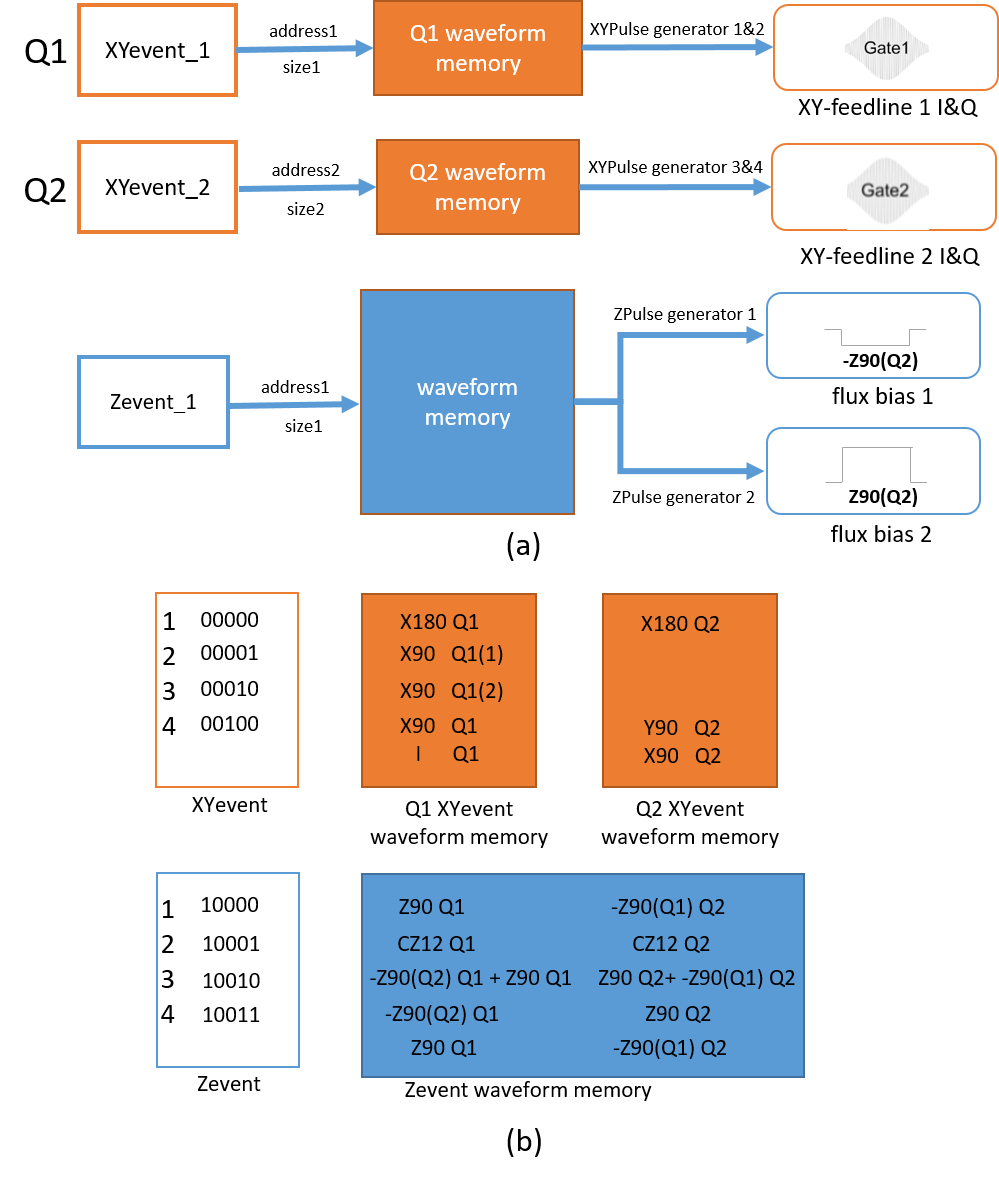
\includegraphics[width=\linewidth]{figure/4_6}
  \caption{overview of electrode event-based microarchitecture}
  \label{img6}
\end{figure}

Considering all quantum operations on the flux bias line require waveform compensation for the superconducting quantum processor as mentioned in Section 2, 
in ebQuMA, all Zevents are described by global events, reducing hardware resource overhead of local Zevent registers and queues. 
As a result, there is n local registers of XYevent and one global register of Zevent in ebQuMA where n is the qubit number. 
When a quantum instruction is executed, the instruction execution module buffers all electrode events with the same timestamp into corresponding event registers according to the event and electrode type. 
Specifically, when a global XYevent operation instruction is executed, the execution module broadcasts the event to every local XYevent register.


The pluse generator unit of ebQuMA is divided according to the electrode type. Limited by hardware resources, 
each waveform generating unit has a maximum of 8 DACs and supports the control of up to 4 qubits of XY electrode or 8 qubits of Z electrode.
The process of decoding events into waveforms and waveform memory model of XY and Zevents are shown in Figure 5. For the XY feedline pulse generator unit, 
each qubit has a separate waveform memory (about 4MB) to store three types of waveforms:
\begin{itemize}
  \item XYevent\_1 is a local event of low-level abstraction that represents single XY-plane rotation quantum gate. 
  The waveform of quantum gate for each qubit needs to be stored in respective waveform memory whose address corresponds to the event code.
  \item XYevent\_2, 3 is also a local event, which is used to represent the waveform of the calibration experiment. 
  In this example, we only calibrate waveform of X90 applied on Q1, thus waveforms only store in the waveform memory of Q1, 
  and the address corresponds to XYevent\_2,3. The waveforms of other qubits in this address space are invalid. 
  If the operand is other qubits, an error will be reported during the compilation phase.
  \item XYevent\_4 is a global event with a higher level of abstraction, which represents electrode events of all qubits in a period of time. 
  Each qubit has a waveform with the same length in the address corresponding to the global event.
\end{itemize}
The XY feedline pulse generator decodes the electrode event of each qubit received from Queue control unit to obtain the address and waveform file size of each event in its own waveform memory, 
and sends it to the corresponding DACs. Each qubit requires two DACs to play two waveforms of In Fhase and Quadrature respectively. Measure pulse generator unit works in the same way as The XY feedline pulse generator, 
except that there is no global event for the measurement.

For the flux bias pulse generator unit, 
All flux bias electrodes share single memory (about 16MB) for waveforms of global event. 
Zevents can be low-level abstractions, such as one Z-rotation gate or a CZ gate, 
corresponding to Zevent\_1,2, or quantum gates applied on different qubits for one timestamp as Zevent\_3, 
or a high-level abstraction of quantum circuits, such as Zevent\_4. When receiving new global event, 
the flux bias pulse generator unit obtains the waveform of each qubit corresponding to the event code from the waveform memory, 
and distributes the waveform file to each DAC through the pulse distribution module.

\subsection{Multi-level Compilation Scheme}

Since quantum applications are described using quantum circuits based on the GATE model, 
while ebQuMA based on electrode events, a multilevel compilation architecture is required to compile quantum applications into ebQuMA executable files. 
It should be noted that mapping between quantum circuit and processor is completed by the top-level compiler, outside the scope of this paper. 
The input circuit of our scheme is optimized and each quantum gate can be directly executed by quantum hardware.
Specifically, the compilation of quantum applications requires the following four steps, as shown in Figure:
\begin{figure}[ht]
  \centering
  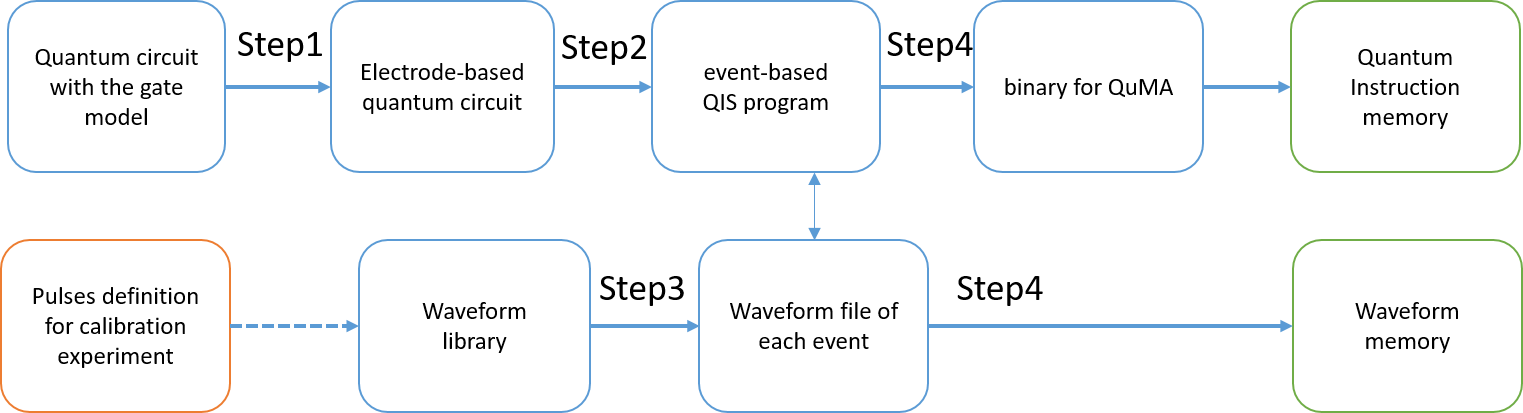
\includegraphics[width=\linewidth]{figure/4_8}
  \caption{overview of electrode event-based microarchitecture}
  \label{img7}
\end{figure}


First, the gate-based quantum circuit is divided into multiple sub-circuits each of which is implemented by one type of electrodes, independently. 
Figure 2.a is the quantum circuit of 3-qubit DJ algorithm. The H-gate is performed by applying one X90 and Z180 gate back to back. 
The circuit is split to two sub-circuits in Figure8. B according to the execution electrode. 
The left part is executed by the XY feedline to implement XY-rotation operation and right one is performed by flux bias lines for Z-rotation and CZ operations. 
I represents the unitary operation and the time axis below the circuit records the initial timestamp of each operation.
\begin{figure}[h]
  \centering
  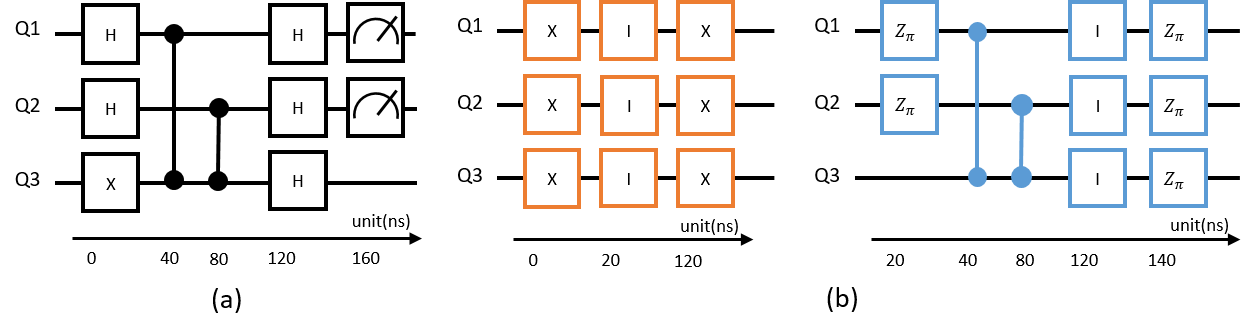
\includegraphics[width=\linewidth]{figure/4_10}
  \caption{overview of electrode event-based microarchitecture}
  \label{img7}
\end{figure}


Secondly, define electrode events with different levels of abstraction according to the characteristics of the quantum circuit for circuit description and use classical instructions to implement program flow control and data transmission. 
When the memory of the pulse generation unit is free enough, low-depth quantum circuits can often be described in high-level abstraction of electrode events. 
The measure instruction divides the quantum program into several sections, and each section is coded with global events the number of which is equal to the independent electrode number. 
The circuit in Figure 9a has only one section. XYGevent1 is used to encode the waveform of the XY feedline for 0-140ns, and for the waveform of the Flux bias line of 20-160ns is stored in Zevent5. 
The quantum program based on ebQIS is shown at the top of Figure 9d.

On the other hand, to save memory overhead, for quantum circuits with low gate diversity, a low-level abstract electrode event description scheme can be used. 
All basic quantum gates implemented by XY feedline are coded as local events. The whole circuit of XY electrode is generated in real time, 
reducing the unitary waveform storage memory and reusing the waveforms of basic gates. For Z electrode events, 
all basic quantum gates performed on single qubit or qubit pairs are encoded with global events, the length of which is the same as quantum gate. 
In addition, the waveforms that frequently multiplexed or with high logic gate density, can also be encoded with global event according to the use of memory. 
Uncoded waveforms is generated by serializing global events of existing single quantum gates.    

The quantum program of example circuit encode with low-level abstraction events is shown in the bottom part of Figure 9d. 
Zevent1-4 represents the waveform of each timestamp of flux bias line when performing quantum gate, 
and XY\_Levent1 for X90 gate. For the specific memory overhead and feasibility of the two schemes, 
we have further discussion in Section 7.


  \begin{algorithm}[ht]
      \caption{caption}
      \begin{ttfamily} 
      \textcolor[RGB]{0,0,205}{SMIS } \quad S1, \{000011\} \\
      0 , \textcolor[RGB]{139,69,19}{XY\_Gevent1}\\    
      1 , \textcolor[RGB]{139,69,19}{Z\_event5}\\
      1 , \textcolor[RGB]{139,69,19}{measure} S1\\
      \textcolor[RGB]{0,0,205}{QWAIT} \quad 30\\
      \textcolor[RGB]{169,169,169}{-------------------------------}\\
      \textcolor[RGB]{0,0,205}{SMIS } \quad S0, \{000111\} \\
      \textcolor[RGB]{0,0,205}{SMIS } \quad S1, \{000011\} \\
      0 , \textcolor[RGB]{139,69,19}{XY\_Levent1} S0\\
      1 , \textcolor[RGB]{139,69,19}{Z\_Levent1}\\
      1 , \textcolor[RGB]{139,69,19}{Z\_Levent2}\\
      2 , \textcolor[RGB]{139,69,19}{Z\_Levent3}\\
      2 , \textcolor[RGB]{139,69,19}{Z\_Levent4}\\
      1 , \textcolor[RGB]{139,69,19}{XY\_Levent1} S0\\
      1 , \textcolor[RGB]{139,69,19}{measure} S1\\
      \textcolor[RGB]{0,0,205}{QWAIT} \quad 30

      \end{ttfamily}
  \end{algorithm} 



The third step is to obtain a waveform file corresponding to each electrode event based on the waveform library and composition of electrode events.
Generally, each quantum processor has a set of calibrated waveforms for basic quantum gates. 
In particular, when the basic quantum gates waveform needs to be recalibrated or there is no pre-stored waveform, the quantum processor needs to execute the calibration procedure first.
For tunable superconducting qubit, there is also a crosstalk matrix used to characterize the crosstalk on flux bias line between each of two qubits. 

The waveform of quantum operation is stored in the form of an one-dimensional array, 
the length of the which depends on the frequency of the DAC and the length of the waveform. 
In the following discussion, we use $\{GATE_i\}$ to represent the waveform file of $GATE_i$. 
The waveforms corresponding to each events of the example are shown in Figure 9.c.

There are two operations of basic waveforms to generate waveform of events: superposition and splicing. 
Waveform superposition is used to obtain the actual waveform of each Z electrode at each timestamp. 
To reduce the effort of crosstalk on flux bias line, 
the actual waveform of one qubit is a linear superposition of its own operation waveform and compensation waveforms of other qubits at the same timestamp, which is expressed assembly
$GATEP_{Qj}= \sum_{i=1,i\neq j}^{n} GATEB_{Qi} \kappa_{ji}+GATEB_{Qj}$. $\kappa_{ji}$ is the coefficient of the crosstalk matrix,  
and $\kappa_{ji}GATE_i$ is the waveform compensation of the qubit i on qubit j, which is denoted as $\{–GATE_{Qi}\}$ in Figure 9.c,  
The superposition of waveform of GATE1 and GATE2 is denoted as $\{GATE_1 + GATE_2\}$.

Waveform splicing that merging multiple waveforms horizontally to get a longer waveform file is used to obtain high-level abstract electrode event waveforms. 
We use $\{\{GATE1\}+\{GATE2\}\}$ to represent waveform splicing of GATE1 and GATE2.
For XY feedline events, a high-level abstract waveform is obtained by stitching basic quantum gates and unitary waveforms according to the composition of XY global event, 
while flux bias electrode event waveform is generated by splicing the waveforms of each timestamp, obtained by waveform superposition.

\newcommand{\tabincell}[2]{\begin{tabular}{@{}#1@{}}#2\end{tabular}}
  \renewcommand\arraystretch{3}
  \begin{table}[ht]  
    \centering  
    \caption{caption}  
    \begin{center}
      \scalebox{0.45}{  
    \begin{tabular}{|c|c|c|c|c|c|c|c|}  
    \hline  
     & Zevent1 & Zevent2 & Zevent3 & Zevent4 & Zevent5 & XY\_Levent1 & XY\_Gevent1 \\ 
     \hline  
     Q1 & \{$Z_{Q1}-Z_{Q2}$\} &  \{$CZ_{Q1,Q3}$\} & \{$-CZ_{Q2,Q3}$\} & \{$Z_{Q1}-Z_{Q2}-Z_{Q3}$\} 
     & \multirow{2}{*}{\tabincell{c}{\{Zevent1+Zevent2\\+Zevent3+Zevent4\\+\{$I_{20}$\}\}}} & \{$X_{Q1}$\} & $\{\{X_{Q1}\}+\{I_{00}\}+\{X_{Q1}\}\}$ \\ 
     \cline{1-5}  \cline{7-8}
     Q2 & \{$Z_{Q2}-Z_{Q1}$\} &  \{$-CZ_{Q1,Q3}$\} & \{$CZ_{Q2,Q3}$\} & \{$Z_{Q2}-Z_{Q1}-Z_{Q3}$\} &  & \{$X_{Q2}$\} & $\{\{X_{Q2}\}+\{I_{00}\}+\{X_{Q2}\}\}$  \\ 
     \cline{1-5}  \cline{7-8}
     Q3 & \{$-Z_{Q1}-Z_{Q2}$\} &  \{$CZ_{Q1,Q3}$\} &  \{$CZ_{Q2,Q3}$\} & \{$Z_{Q3}-Z_{Q1}-Z_{Q2}$\}  &  & \{$X_{Q3}$\} & $\{\{X_{Q3}\}+\{I_{00}\}+\{X_{Q3}\}\}$  \\
     \hline
     Duration & $20ns$ & $40ns$ & $40ns$ & $20ns$ & $140ns$ & $20ns$ & $140ns$  \\ 
    \hline  
    \end{tabular}} 
    \end{center}  
    \end{table}

Finally, matching the electrode event code with the storage address of the pulse generation unit. 
Since the length of global events are not constant, it is necessary to include not only the waveform address, but the size of the waveform file in the event encoding. 
We pre-defined the mapping relationship between the event encoding and the waveform file size and address, and write in ebQuMA as a lookup table. 
When compiling different quantum applications, the event coding adopts the established scheme. 
Therefore, only the waveform file and micro-architecture program need to be reloaded when performing different quantum applications, 
without modifying the architecture of ebQuMA. However, memory fragmentation will occur, resulting in low memory utilization. 
Another solution is to re-program the look-up table of the event code and waveform information when loading quantum program, increasing the efficiency of memory usage, 
at the cost of uploading time. The choice between the two schemes depends on the demand for memory resources.
\section{implementation}
\begin{figure*}[ht]
  \centering
  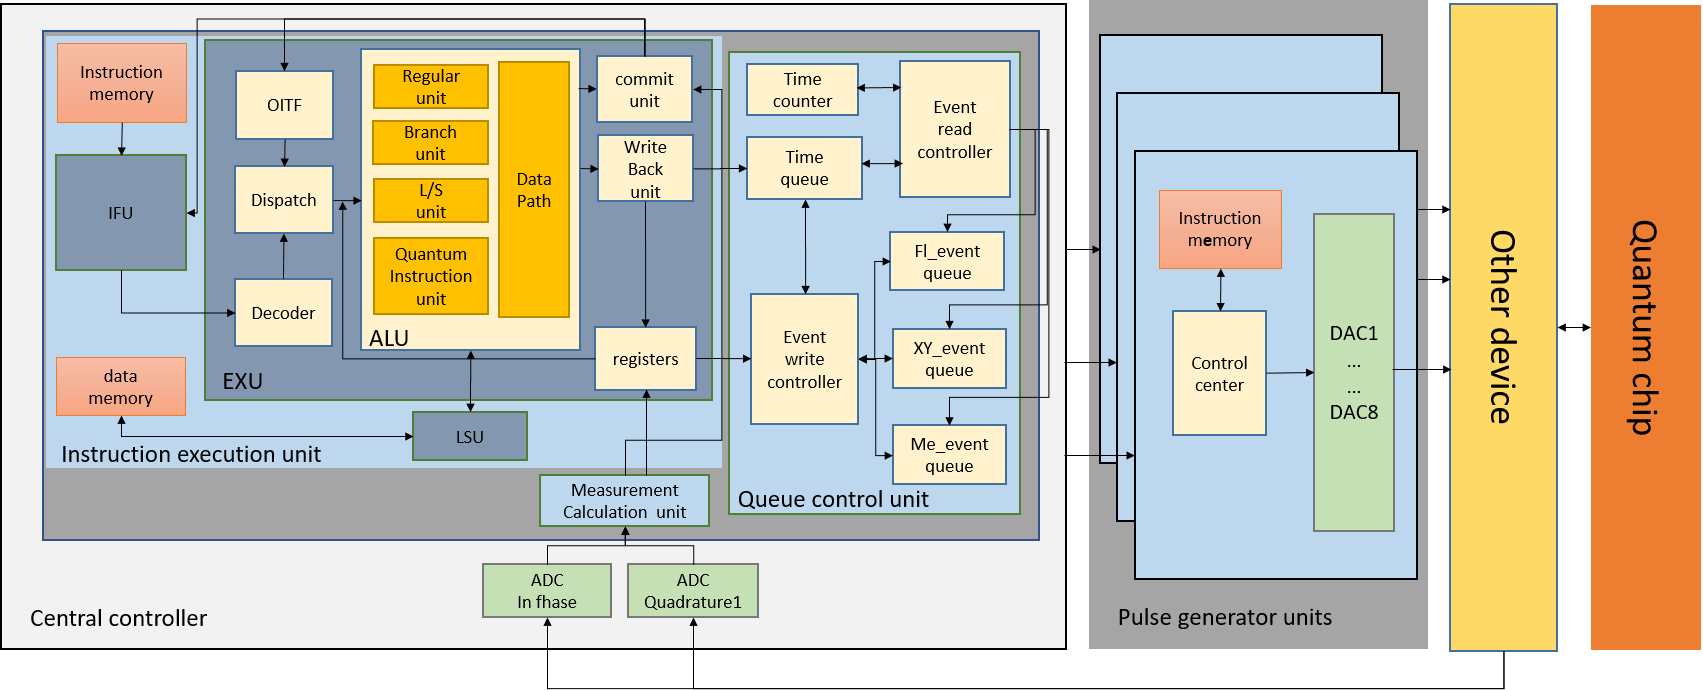
\includegraphics[width=\linewidth]{figure/5_1}
  \caption{overview of electrode event-based microarchitecture}
  \label{img7}
\end{figure*}
In this Section, we discuss the implementation of ebQuMA. ebQuMA consists of a central controller and multiple waveform generation units, 
as shown in Figure 10. The central controller is implemented using an Arrow BeMicroCV A9 board holding an Altera Cyclone V 5CEFA9 FPGA chip, 
connects to two 8-bit resolution analog-to-digital converters (ADC) to digitize analog measurement signals. 
The central controller consists of instruction execution unit, queue control unit, and measurement calculation unit. 
The clock frequency of the instruction execution unit is 100MHz, and 50MHz for Queue control unit.

The instruction execution unit is a two-stage pipelined processor architecture. 
Since the encoding format of quantum instructions in ebQIS is the same as the classical instruction, 
they are executed at the same stage. The instruction fetch unit (IFU) reads the instruction from the instruction memory and sends it to the execution unit (EXU). 
The Exu decodes and checks the data and resource correlation through the outstanding instruction track fifo (OITF). If there is a conflict, the pipeline is blocked. 
In addition to the classic WAW, WAR, and RAW conflicts, when the dispatched instruction is FMR or Measure but the last measurement result of the target qubit is not returned, 
a conflict also occurs, until the measurement result is returned. At the same time, when instructions are dispatched, 
the entries of potentially conflicting instructions are stored in the OITF, 
Such as target qubit of measure instruction and the destination register index of Load instruction.
If there is no conflict, the dispatch module will send it to one of the four unit of the arithmetic and logic unit according to the instruction type, 
which are used to perform arithmetic logic operations, branch instructions, storage instructions and quantum instructions respectively, 
and reuse the same data path for calculation.

Here, we only introduce the execution process of quantum instructions.
If the PI of the quantum instruction is 0, the electrode event coding of up to two quantum operations in the current 
instruction are added to the value of the event register of target qubit (for XY feedline local event) or the global event register (for flux bias line event). 
For the global event of XY feedline, the XY feedline event register for each qubit is added to the event coding. 
The event register is used to buffer the event of each electrode with the same timestamp. 
If PI is not zero, the event of the current instruction is written to the corresponding event register, 
and rest of event registers are set to zero. At the same time, a new timestamp is calculated by data path. 
As for the Qwait, FMR, and SMIS instructions, the execution method is similar to the ADD instruction, except that the source and destination registers are different. 

The write back unit (WBU) update registers with the calculation results from ALU. 
If the current instruction generates a new timestamp, the WBU sends the value of all event registers to the queue control module, 
as well as the new timestamp. The commit unit is responsible for pipeline flushing and update of entries in the OITF. 
After complete the write back of Load instruction or measurement instruction, the entries in the OITF are cleared by the commit unit. 
The LSU module is used for data interaction with the data memory.

The queue control unit realizes precise time control of the quantum processor. The queue writing controller buffers the timestamp and event sent by the instruction execution unit to the corresponding electrode event queue and time queue. 
When a trigger signal is received, the time counter starts counting. If the counter is equal to the head element of the time queue, the electrode events corresponding to this timestamp are sent to the pulse generator units by the event read controller. 

In particular, when there is only one element left in the time queue and the value of the time counter is equal to it, 
To prevent timing errors, the time counter will suspend counting until a new timestamp is received. At the same time, 
the event read controller sends the accepted electrode event (event corresponding to the last timestamp in time queue) directly to the pulse generator unit through the bypass.
This situation occurs when the instruction execution module needs to execute more instructions to obtain electrode events at the next point in time, 
so that all buffered events have been executed, mainly in feedback programs based on measurement results.

Although this scheme will cause the applied waveform not to strictly follow the timing specified by the instruction, 
in fact, for quantum applications, it is only necessary to ensure that the execution time interval of two quantum gates is not less than the duration time of the first quantum gate to avoid error.
For the circuit that need to be executed strictly in accordance with timing, 
such as calibration experiments, high-level abstraction of electrode event can be used. 
Since the instruction execution time is much shorter than the waveform length, this situation will not occur.

The measurement calculation unit (MCU) analyzes and processes the measurement waveforms of the qubits collected by the ADCs to obtain the states of target qubits. 
For more detail about measurement discrimination using a customized FPGA, please refer to []. 
When the qubit status is obtained, the MCU updates the qubit measurement result register and submits an application for measurement completion to the commit unit.


\section{evaluation}
\section{conclusion}


\bibliographystyle{plain}
\bibliography{bib/wpref}

\end{document}

\endinput